\documentclass[../../Instructions_Framework]{subfiles}
% Hier müssen keine Packages geladen werden, es werden automatisch die von masterdoc geladen,
% sowie die Konfigurationen.
% Bei includegraphics nur Bildname (Bsp: Bild.png) eingeben, da er in den angegebenen Pfade die Bilder sucht
\graphicspath{{img/}{img/}}
\begin{document}
\chapter{Instructions for creating scenes}
The following chapter shows the creation of a scene in Unity. The requirements are Unity version 5.5.1f and the BullsEye.unitypackages.\\
\section{Select your reality}
Depending on whether you want to create an augmented or a virtual reality scene you have two distinct prefabs which can be used.
\subsection{Augmented Reality}
The \textit{AR} prefab is used for augmented reality scenes. The prefab can be found in the Asset Folder under the data path \textbf{Assets/BullsEye/Prefabs}. To create a scene you need to drag and drop the prefab into the hierarchy. This will setup every required render component (see Fig. \ref{fig:screenshot002}).
\begin{figure}
	\centering
	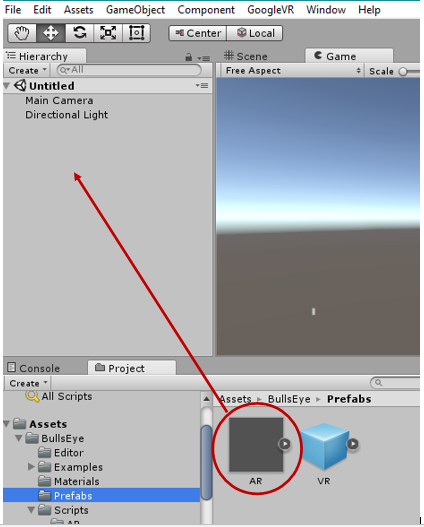
\includegraphics[width=0.7\linewidth]{img/screenshot002}
	\caption{AR prefab}
	\label{fig:screenshot002}
\end{figure}
The AR prefab differs from the VR prefab by including a plane which acts as a \textit{screen} and displays the real world as a video stream. If you switch to scene view you can see the basic AR scene setup, consisting of the camera and the \textit{screen} to show the video stream of the real world. You are now set up to include your own objects into the scene to augment the reality displayed on the plane (see Fig. \ref{fig:screenshot004}).
\begin{figure}
	\centering
	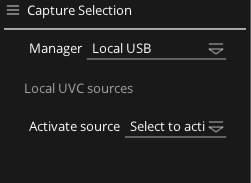
\includegraphics[width=0.7\linewidth]{img/screenshot004}
	\caption{AR prefab structure}
	\label{fig:screenshot004}
\end{figure}

\subsection{Virtual Reality}
The \textit{VR} prefab can be used for virtual reality. The prefab can be found in the Asset Folder under the data path \textbf{Assets/BullsEye/Prefabs}. To create a scene you need to drag and drop the prefab into the hierarchy. This will setup every required render component (see Fig. \ref{fig:screenshot003}).
\begin{figure}
	\centering
	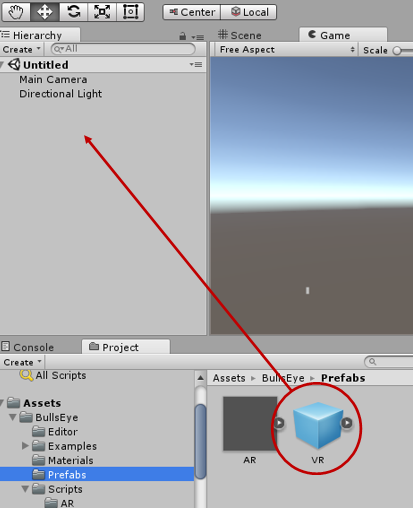
\includegraphics[width=0.7\linewidth]{img/screenshot003}
	\caption{VR prefab}
	\label{fig:screenshot003}
\end{figure}
To create a virtual reality scene you simply need to create a new scene (see Fig. \ref{fig:screenshot005}), but instead of dragging the AR prefab into the hierarchy as explained before, you will instead drag the VR prefab into the hierarchy. You are now ready to build your virtual world around the prefab. Fig. \ref{pic8} show the VR prefab in an example virtual reality scene.
\begin{figure}
	\centering
	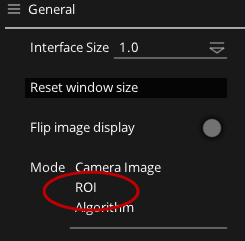
\includegraphics[width=0.7\linewidth]{img/screenshot005}
	\caption{VR prefab structure}
	\label{fig:screenshot005}
\end{figure}

\begin{figure}[htp]
	\centering
	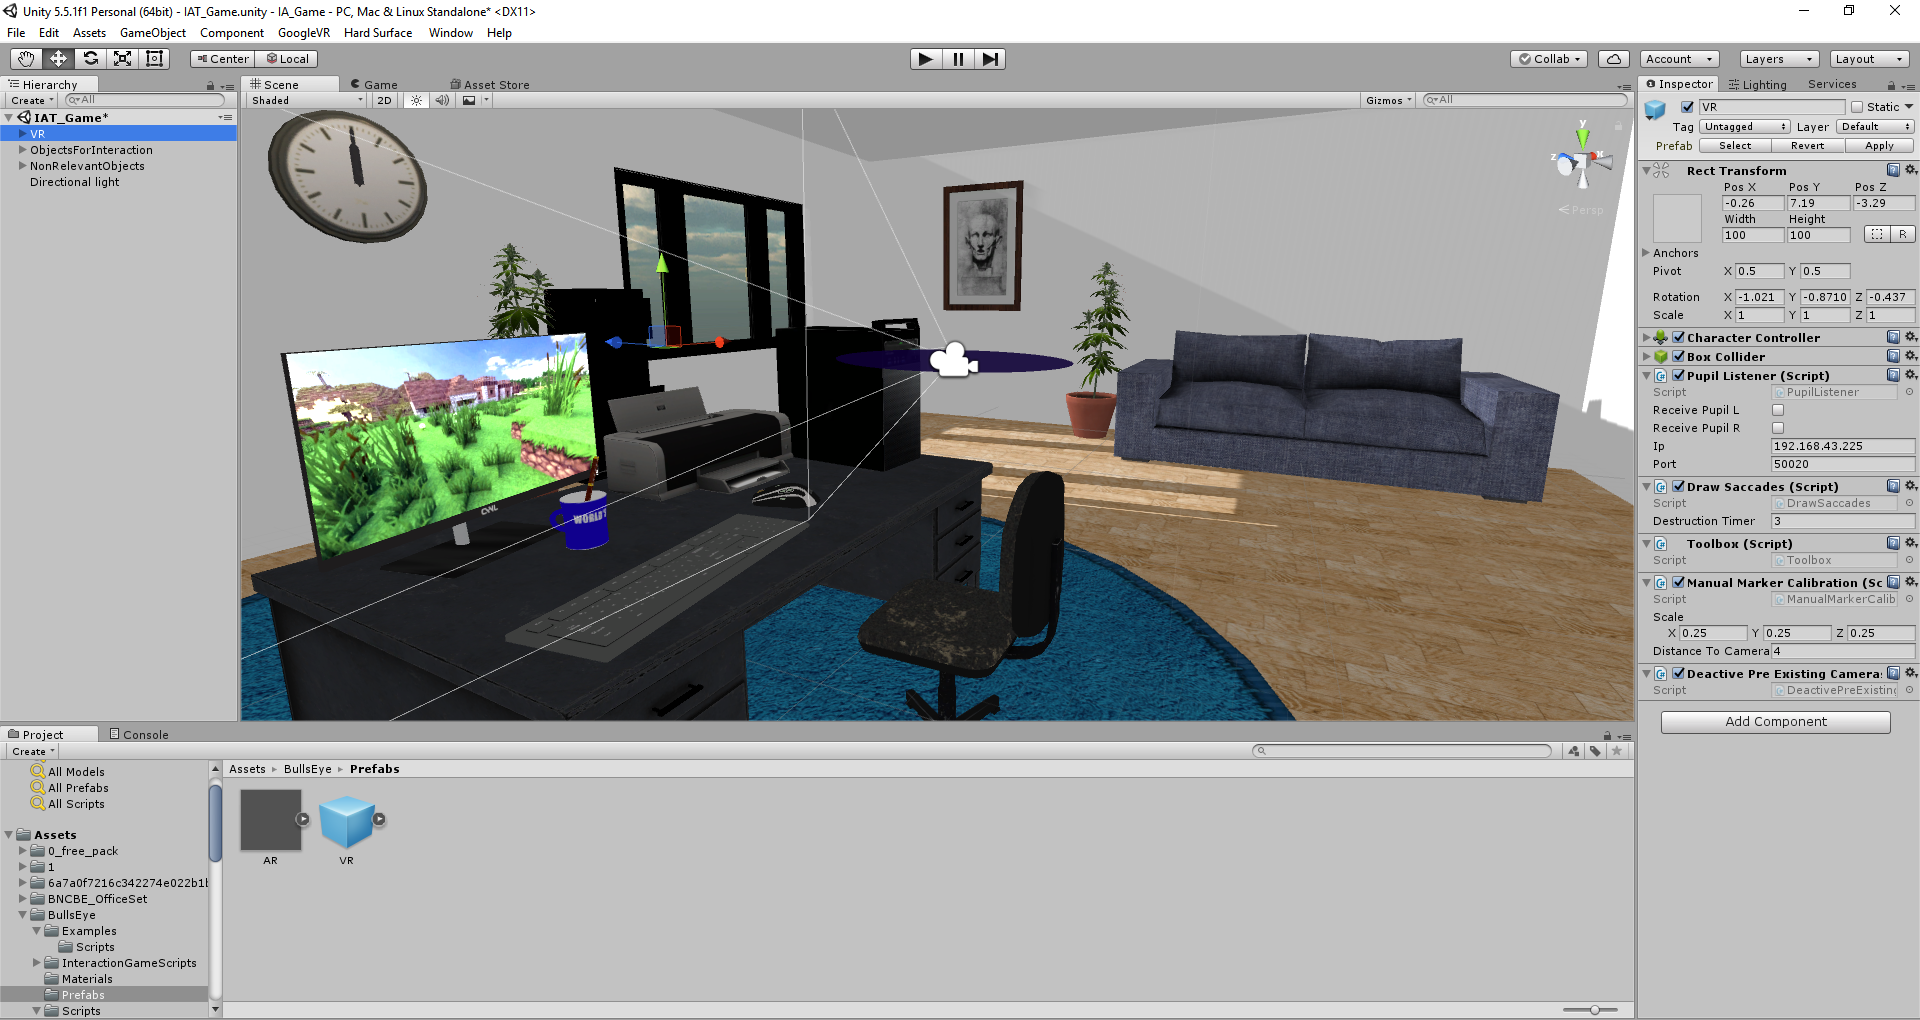
\includegraphics[width=1.0\linewidth]{pic7.png}
	\caption{The VR prefab in an example VR scene}
	\label{pic8}
\end{figure}
After creation your scene go to chapter \ref{usage} for use an existing example interaction technique or to chapter \ref{technique} for creation your own interaction technique.

\end{document}